
\de{ĐỀ THI GIỮA HỌC KỲ I NĂM HỌC 2023-2024}{THPT Nguyễn Chí Thanh}
\Opensolutionfile{ans}[ans/ans]
\Closesolutionfile{ans}
\setcounter{bt}{0}
%Câu 1a...........................
\begin{bt}%[1D1B2-2]%[Dự án đề kiểm tra Toán 11 GHKI NH23-24- Đoàn Minh Tâm]%[THPT Nguyễn Chí Thanh- Tp HCM]
	Cho $\sin \alpha=\dfrac{12}{13}$ và $\dfrac{\pi}{2}<\alpha<\pi$. Hãy tính $\cos \alpha$, $\cos \left(\dfrac{\pi}{3}-\alpha\right)$.
	\loigiai{
		Do $\dfrac{\pi}{2}<\alpha<\pi$ nên $\heva{&\sin x>0\\&\cos x <0.}$\\
		Ta có $\sin^2\alpha+\cos^2\alpha=1 \Leftrightarrow \cos^2x =\dfrac{25}{169} \Leftrightarrow \hoac{&\cos x =-\dfrac{5}{13} &\text{(nhận)}\\&\cos x=\dfrac{5}{13} &\text{(loại)}.}$\\
		Ta có $\cos \left(\dfrac{\pi}{3}-\alpha\right)=\cos\dfrac{\pi}{3}\cos\alpha + \sin\dfrac{\pi}{3}\sin\alpha=\dfrac{-5+12\sqrt{3}}{26}$.
	}
\end{bt}

%Câu 1b..........................
\begin{bt}%[1D1B4-1]%[Dự án đề kiểm tra Toán 11 GHKI NH23-24- Đoàn Minh Tâm]%[THPT Nguyễn Chí Thanh- Tp HCM]
	Tìm tập xác định của hàm số $y=\cot \left(2 x-\dfrac{\pi}{3}\right)$.
	\loigiai{Điều kiện xác định $2 x-\dfrac{\pi}{3} \ne k\pi \Leftrightarrow x \ne \dfrac{\pi}{6}+k\dfrac{\pi}{2}$ ($k\in \mathbb{Z}$).\\
		Vậy tập xác định là $\mathscr{D}=\mathbb{R}\setminus\left\lbrace \dfrac{\pi}{6}+k\dfrac{\pi}{2} \mid k \in \mathbb{Z} \right\rbrace$.
	}
\end{bt}

%Câu 1c..........................
\begin{bt}%[1D1Y1-2]%[Dự án đề kiểm tra Toán 11 GHKI NH23-24- Đoàn Minh Tâm]%[THPT Nguyễn Chí Thanh- Tp HCM]
	Giải phương trình $2 \cos \left(2 x-\dfrac{\pi}{3}\right)+1=0$.
	\loigiai{
		Ta có
		\begin{eqnarray*}
			&& 2 \cos \left(2 x-\dfrac{\pi}{3}\right)+1=0\\
			&\Leftrightarrow & \cos \left(2 x-\dfrac{\pi}{3}\right)=-\dfrac{1}{2}\\
			&\Leftrightarrow & \hoac{&2 x-\dfrac{\pi}{3}=\dfrac{2\pi}{3}+k2\pi\\&2 x-\dfrac{\pi}{3}=-\dfrac{2\pi}{3}+k2\pi}\\
			&\Leftrightarrow & \hoac{&x=\dfrac{\pi}{2}+k\pi\\&x=-\dfrac{\pi}{6}+k\pi} (k \in \mathbb{Z}).
		\end{eqnarray*}
		Vậy $S=\left\{\dfrac{\pi}{2}+k\pi;-\dfrac{\pi}{6}+k\pi\mid k \in \mathbb{Z}\right\}$.
	}
\end{bt}

%Câu 2a..........................
\begin{bt}%[1D1B1-3]%[Dự án đề kiểm tra Toán 11 GHKI NH23-24- Đoàn Minh Tâm]%[THPT Nguyễn Chí Thanh- Tp HCM]
	\immini{
		Viết công thức số đo tổng quát của các góc lượng giác $(O A, O M)$ và $(O A, O N)$ trong hình bên.
	}{
		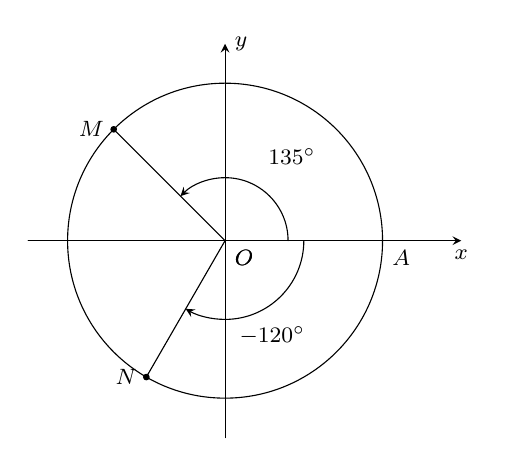
\begin{tikzpicture}[scale=1, font=\footnotesize, line join=round, line cap=round, >=stealth]
			\draw[-stealth] (-2.5,0) -- (3,0)node[below] {$x$};
			\draw[-stealth] (0,-2.5) -- (0,2.5)node[right] {$y$};
			\draw[black] (0,0) circle (2);
			\draw[-stealth] (0:.8) arc (0:135:.8);
			\draw[-stealth] (0:1) arc (0:-120:1);
			\draw[fill=black] (0:0) node[below right]{$O$}--(135:2) circle(1pt) node[left]{$M$};
			\draw[fill=black] (0:0) node[below right]{$O$}--(-120:2) circle(1pt) node[left]{$N$};
			\path (-60:1.2) node[below=-2pt]{$-120^{\circ}$};
			\path (45:1.2) node[above]{$135^\circ$};
			\path (0:2) node[below right]{$A$};
		\end{tikzpicture}
	}
	\loigiai{
		\begin{itemize}
			\item $(O A, O M)=135^\circ + k 360^\circ$ ($k \in \mathbb{Z}$).
			\item $(O A, O N)=-120^\circ +k360^\circ$ ($k \in \mathbb{Z}$).
		\end{itemize}
	}
\end{bt}

%Câu 2b..........................
\begin{bt}%ID%[Dự án đề kiểm tra Toán 11 GHKI NH23-24- Đoàn Minh Tâm]%[THPT Nguyễn Chí Thanh- Tp HCM]
	\immini{Trên đồng hồ có kim chỉ giờ dài $6 $ cm có gắn một con rùa ở đầu kim và kim chỉ phút dài $11$ cm có gắn một con thỏ ở đầu kim. Tại thời điểm quan sát đồng hồ đang chỉ $4$ giờ đúng. Tính hiệu quãng đường của thỏ và rùa đi được tính từ lúc $4$ giờ đúng đến $5$ giờ đúng.}{
		
\begin{tikzpicture}[scale=0.3]
			\def\hours{0}
			\def\minutes{0}
			\def\seconds{0}
			\draw[line width=0.2cm] (0,0) circle (5.1cm);
			% Minutes
			\foreach \i in {1,2,...,60}{
				\def\angle{\i*6}
				\draw[thin] (\angle:5cm) -- (\angle:4.9cm);
			}
			
			% 5 minutes
			\foreach \i in {1,2,...,12}{
				\def\angle{\i*-30+90}
				\draw[thin] (\angle:5cm) -- (\angle:4.5cm);
				\node at (\angle:4cm) {\i};
			};
			
			% Hour hand
			\def\angle{\hours*-30 + \minutes*-0.5 + \seconds*-0.008333 -180}
			\draw[line width=0.1cm] (0,0) -- (-30:2.5cm);
			
			% Minute hand
			\def\angle{\minutes*-6 + \seconds*-0.1 +90}
			\draw[line width=0.05cm] (0,0) -- (\angle:4cm);
			
			%% Second hand
			% \def\angle{\seconds*-6+90}
			% \draw[very thick,color=red] (\angle:-1cm) -- (\angle:4.5cm);
			% \draw[line width=0.1cm,color=red] (\angle:-1cm) -- (\angle:-0.25cm);
			
			% Center dot
			\draw[fill=black] (0,0) circle (0.1cm);
		\end{tikzpicture}
	}
	\loigiai{
		Ta có đồng hồ được chia thành $12$ phần bằng nhau nên mỗi phần là $\dfrac{360^\circ}{12}=30^\circ$.\\
		Kim giờ quay được một giờ thì quãng đường con rùa đi được là $\dfrac{\pi \cdot 6 \cdot 30^\circ}{180^\circ}=\pi$.\\
		Kim phút sau mộ giờ quay được 1 vòng nên quãng đường con thỏ đi được là $2\pi \cdot 11=22\pi$.\\
		Vậy hiệu quãng đường đi được là $22\pi - \pi =21 \pi$.
	}
\end{bt}
\begin{bt}%[1D1K3-4]%[Dự án đề kiểm tra Toán 11 GHKI NH23-24- Hiếu Mai]%[THPT Nguyễn Chí Thanh - Tp HCM]
	\begin{listEX}[1]
		\item Chứng minh biểu thức sau không phụ thuộc vào giá trị của $x$
		$$
		P=\sin \left(\dfrac{\pi}{2}-x\right)+\cos (\pi+x)-\tan \left(\dfrac{\pi}{2}-x\right) \tan (\pi-x).
		$$
		\item Chúng minh rằng: $\dfrac{\sin \alpha+\cos \alpha}{\sin ^3 \alpha}=\dfrac{1-\cot ^4 \alpha}{1-\cot \alpha}$ với mọi $\alpha \neq k \pi, \alpha \neq \dfrac{\pi}{4}+k \pi, k \in \mathbb{Z}$
	\end{listEX}
	\loigiai{
		\begin{listEX}[1]
			\item Ta thấy
			\begin{align*}
				P&= \cos x - \cos x - \cot x \cdot (-\tan x)
				\\
				&= \cot x \cdot \tan x
				\\
				&= 1.
			\end{align*}
			Nên $ P $ không phụ thuộc vào giá trị của $x$.
			\item Do
			\begin{align*}
				\dfrac{1-\cot ^4 \alpha}{1-\cot \alpha} 
				&= \dfrac{(1-\cot\alpha)(1+\cot\alpha)(1+\cot^2\alpha)}{1-\cot\alpha}
				\\
				&= \left(1+ \dfrac{\cos\alpha}{\sin\alpha}\right) \cdot \dfrac{1}{\sin^2\alpha}
				\\
				&= \dfrac{\sin \alpha+\cos \alpha}{\sin ^3 \alpha}
			\end{align*}
			Ta được điều phải chứng minh.
		\end{listEX}
	}
\end{bt}
%Câu 4...........................
\begin{bt}%[1D1T5-6]%[Dự án đề kiểm tra Toán 11 GHKI NH23-24- Hiếu Mai]%[THPT Nguyễn Chí Thanh - Tp HCM]
	\immini
	{Một chiếc guồng nước có dạng hình tròn tâm $O$ bán kính $2{,}5$m, trên guồng nước có gắn một chiếc gàu múc nước; trục của guồng nước đặt tại $O$ cách mặt nước $2$m (hình bên). Biết rằng guồng nước quay đều theo chiều ngược chiều kim đồng hồ với tốc độ 1 vòng/phút. Giả sử ban đầu chiếc gàu múc nước ở vị trí $M$, sau $t$ phút $(t>0)$ guồng quay chiếc gàu múc nước đến vị trí điểm $A$. Gọi $h$ (mét) là khoảng cách tính từ điểm $A$ trên guồng nước đến mặt nước.}
	{
		\begin{tikzpicture}[
			>=stealth, line join=round, line cap=round, 
			scale=1, %rotate=90,
			declare function={a=2.5; p=60;}]
			% ve diem
			\path 
			(0,0) coordinate (o)
			(0:a) coordinate (M)
			(180:a) coordinate (E)
			(-90:2) coordinate (N)
			(60:a) coordinate (A)
			;
			\draw [name path=dtO]  (0,0) circle (a);
			
			\draw[fill=blue] (0,0) node[shift={(180:.5)}] {$ O $} circle (2pt) -- (M) circle (2pt) node[shift={(0:.5)}] {$ M $};
			\draw[fill=blue, <->] (0,0) -- (A) circle (2pt) node[shift={(60:.5)}] {$ A $} node[pos=.5, sloped, above] {$ 2,5 $m};
			\draw[dashed]
			(-2.5,-2) node[] (n1) {}-- (2.5,-2) node[] (n2) {}; 
			\draw[dashed, <->] (A) -- ($ (n1)!(A)!(n2) $) node[pos=.3, right] {$ h $};
			\draw[dashed, <->] (o) -- (N) node[pos=.5, left] {$ 2 $m};
			%	\node[anchor=south] at (90:{1.1*a}) {$ abc $};
			\node[] at (0,-3) {Mô phỏng guồng nước};
		\end{tikzpicture}
	}
	\begin{listEX}[1]
		\item Hãy lập công thức tính $h(m)$ theo thời gian $t$ (phút) tính từ
		khi gàu bắt đầu quay từ vị trí $ M $. (Quy ước nếu $h>0$ thì gàu múc ở trên mặt nước, nếu $h<0$ thì gàu múc ở dưới mặt nước).
		\item Tính các thời điểm gàu đạt độ cao lớn nhất so với mặt nước.
	\end{listEX}
	\loigiai{
		\begin{center}
			\begin{tikzpicture}[
				>=stealth, line join=round, line cap=round, 
				scale=1, %rotate=90,
				declare function={a=2.5; p=60;}]
				% ve diem
				\path 
				(0,0) coordinate (o)
				(0:a) coordinate (M)
				(180:a) coordinate (E)
				(-90:2) coordinate (N)
				(60:a) coordinate (A)
				(0:{a/2}) coordinate (K)
				;
				\draw [name path=dtO]  (0,0) circle (a);
				
				\draw[fill=blue] (0,0) node[shift={(180:.5)}] {$ O $} circle (2pt) -- (M) circle (2pt) node[shift={(0:.5)}] {$ M $};
				\draw[fill=blue, <->] (0,0) -- (A) circle (2pt) node[shift={(60:.5)}] {$ A $};
				\draw[dashed]
				(-2.5,-2) node[] (n1) {}-- (2.5,-2) node[] (n2) {}; 
				\draw[dashed, <->] (A) -- ($ (n1)!(A)!(n2) $);
				\draw[dashed, <->] (o) -- (N);
				\foreach \x/\g in {N/135, K/45}{
					\draw[fill=black] (\x) circle (1.5pt)+(\g:.4) node{$\x$};}
			\end{tikzpicture}
		\end{center}
		\begin{listEX}[1]
			\item Mỗi phút gàu quay được một vòng $ (2\pi \text{ rad}) $ nên góc quay $ \widehat{MOA} $ tại thời điểm $ t $ phút là
			$$
			\widehat{MOA} = (2\pi) \cdot t = 2\pi t.
			$$
			Chiều cao $ h $ của gàu so với mặt nước
			$$
			h = ON + AK
			= ON + OA \cdot \sin\widehat{MOA}
			= 2 + 2{,}5\sin(2\pi t).
			$$
			\item Gàu đạt độ cao lớn nhất so với mặt nước khi 
			$$
			h_\text{max} = 2 + 2{,}5 = 4{,}5.
			$$
			khi 
			$$
			\sin(2\pi t) = 1
			\Leftrightarrow
			2\pi t = \dfrac{\pi}{2} + k\cdot 2\pi
			\Leftrightarrow
			t = \dfrac{1}{4} + k
			\quad (k \in \mathbb{N}).
			$$
			Vậy các thời điểm gàu nước đạt độ cao lớn nhất so với mặt nước là $ t = \dfrac{1}{4} + k \quad (k \in \mathbb{N}) $.
		\end{listEX}
	}
\end{bt}

%Câu 5...........................
\begin{bt}%[1H1K2-4]%[Dự án đề kiểm tra Toán 11 GHKI NH23-24- Nguyễn Sơn]%[THPT Nguyễn Chí Thanh - Tp HCM]
Cho hình chóp $ S.ABCD $, $ ABCD $ là hình thang có đáy là $ AD $ và $ BC $, $ AD = 2BC $.
Gọi $ E $ là trung điểm $ SA $, $ M $ là trọng tâm $ \triangle SAD $, $ G $ là giao điểm của $ AC $ và $ BD $.
\begin{listEX}[1]
	\item Tìm giao tuyến của hai mặt phẳng $ (MBC) $ và $ (SAD) $.
	\item Tìm $ F $ là giao điểm của $ MC $ và mặt phẳng $ (SBD) $.
	\item Chứng minh $ MG $ song song với $ BE $.
\end{listEX}
\loigiai{
\begin{center}
\begin{tikzpicture}[
	>=stealth, line join=round, line cap=round, 
	scale=1,
	declare function={r=3; a=75;}]
% ve diem
	\path 
		(0,0) coordinate (A)
		(-3,-3) coordinate (B)
		(2,-3) coordinate (C)
		(10,0) coordinate (D)
		(-1,6) coordinate (S)
		($ (S)!.5!(A) $) coordinate (E)
		($ (E)!{1/3}!(D) $) coordinate (M)
		(intersection of A--C and B--D) coordinate (G)
		($ (S)!{2/3}!(A) $) coordinate (H)
		($ (S)!{2/3}!(D) $) coordinate (K)
		(intersection of B--K and M--C) coordinate (F)
		;
	\draw[thick] 
		(S)--(B)--(C)--(D)--(S)--(C)
		;
	\draw[dashed]
		(S)--(A)--(B)--(D)--(E)
		(D)--(A)--(C)--(M)--(B)
		(H)--(K)--(B);
% phan giac goc A
%	\path[name path=t1] (A) -- (B) -- (C) -- cycle;
%	\path[name path=c1] (A) circle (2);
%	\path[name intersections={of = c1 and t1, by={a,b}}];
%	\path 
%		($ (a)!.5!(b) $) coordinate (d)
%		(intersection of A--d and B--C) coordinate (D);
% ve duong tron
%	\draw [name path=dtO]  (O) circle (r);
% giao diem cua duong tron voi duong tron/duong thang
%	\path[name intersections={of= dtO and dtI}] coordinate (B) at (intersection-1)  coordinate (C) at (intersection-2); 
% hinh chieu vuong goc cua B len AC
%	\path ($(A)!(B)!(C)$) coordinate (E);
% giao diem cua doan thang voi doan thang
%	\path (intersection of O--S and C--B) coordinate (M);
% danh dau goc
	\foreach \a/\b/\c in {}	{
		\draw pic [draw=black,angle radius = 10] {right angle = \a--\b--\c};
	}
%	\draw pic ["$1$", draw, angle eccentricity=1.3, angle radius=20] {angle = B--A--C};
% danh dau diem
	\foreach \x/\g in {S/90, A/135, B/-135, C/-45, D/0, E/135, M/45, G/-90, H/180, K/45, F/135}{
		\draw[fill=black] (\x) circle (1.5pt)+(\g:.4) node{$\x$};}
\end{tikzpicture}
\end{center}
\begin{listEX}[1]
	\item Xét hai mặt phẳng $ (MBC) $ và $ (SAD) $, ta thấy
	$
		\heva{
			&M \in (MBC)\cap (SAD)\\
			&BC \subset (MBC)\\
			&AD \subset (SAD)\\
			&AD \parallel BC
		}
	$
	\\
	$ \Rightarrow $ giao tuyến của $ (MBC) $ và $ (SAD) $ là đường thẳng qua $ M $, song song với $ AD $ và $ BC $, cắt $ SA $ và $ SD $ lần lượt tại $ H $ và $ K $.
	\item Trong mặt phẳng $ (MBC) $, gọi $ F $ là giao điểm của $ BK $ và $ MC $.
	Ta thấy	$\heva{&F \in MC \\ &F \in BK \subset (SBD) }	$
	\\
	Suy ra $ F $ là giao điểm của $ MC $ và mặt phẳng $ (SBD) $.
	\item $ \triangle GBC $ đồng dạng $ \triangle GDA $ cho ta
	$\dfrac{GB}{GD} = \dfrac{BC}{AD} = \dfrac{1}{2} \quad (1)$.\\
	$ M $ là trọng tâm $ \triangle SAD $ nên $\dfrac{ME}{MD} = \dfrac{1}{2} \quad (2)$.\\
	Từ $ (1) $ và $ (2) $ suy ra $ \dfrac{GB}{GD} = \dfrac{ME}{MD} $. 
	\\
	Do vậy theo định lý Thalet đảo, ta có $ MG \parallel BE$.
\end{listEX}
}
\end{bt}

